%----------------------------------------------------------------------------
\chapter{Felsőszintű architektúra}
\label{sec:Architecture}
%----------------------------------------------------------------------------

Ebben a fejezetben bemutatom a szoftver felépítését.  
Ez a rész elsősorban az architektúrális és programszervezési megoldásokra fókuszál.  
Hasonlóan a \refstruc{sec:Sepcification} fejezethez, ez is csak egy átfogó képet ad a szoftverről, a részletekbe nem merül el.

\section{High-level architektúra}
\label{sec:HighLevelArchitecture}

Ez az alfejezet bemutatja a forráskód szervezését és a legfontosabb követett tervezési mintákat.

\subsection{A program struktúrális szervezése}

Ez a rész a kód forrásfájlokba szervezését mutatja be.  
A hatékony munkához elengedhetetlen egy jól felépített és követett mintát konzisztensen alkalmazni a fejlesztés során.

\subsubsection{A Kotlin Multiplatform alkalmazások felépítése}

Minden Kotlin Multiplatform projekt tartalmaz legalább 3 fő könyvtárat az src mappán belül.  
Szükséges egy commonMain mappa, amely a közös kódrészleteket tartalmazza. Minél több tartalom található ebben megvalósítva, és nem külön kiszervezve, annál jobb a kód újrafelhasználhatósága.  
A többi fő mappa a platform-specifikus kódrészleteket tartalmazza. Az én alkalmazásomban van egy androidMain és egy desktopMain, ezek a jvmMain-nek felelhetők meg.  
Sajnos eszközhiány miatt iOS-re nem tudtam elkészíteni az alkalmazást, mivel annak lefordításához szükség van egy Mac számítógépre.

\begin{figure}[!ht]
    \centering
    \begin{tabular}{cc} % Három oszlop és két sor elrendezése
        % Első sor
        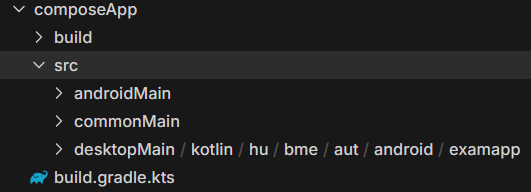
\includegraphics[width=0.35\textwidth, keepaspectratio]{figures/KmpFileStructure.png} & 
        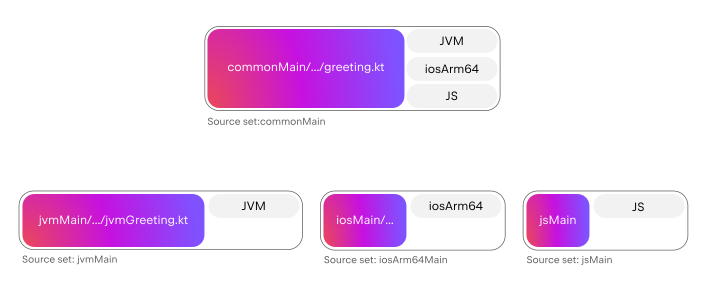
\includegraphics[width=0.65\textwidth, keepaspectratio]{figures/specific-target-diagram.png}
    \end{tabular}
    \caption{Fájl struktúrája az alkalmazásnak. Második kép: \cite{BasicProject}}
    \label{fig:FileStructure}
\end{figure}

A build megfelelő működéséért a Run Configurations fájlok és a build.gradle.kts fájlok felelnek.
A gradel fájlokban kell a függőségeket megadni, a verziók támogatására használható a libs.version.toml fájl.

A \ref{fig:FileStructure}.~ábrán is látható a build.gradle.kts fájlt (\ref{lst:Gradle}.~kódrészlet) is. Az ebben lévő Kotlin DSL-lel létrehozott Gradlenek is tükrözni kell ezt a felépítést.

\begin{lstlisting}[caption={build.gradle.kts fájl struktúrája}, label={lst:Gradle}, language=Kotlin]
import org.jetbrains.compose.desktop.application.dsl.TargetFormat //Importok
...
//Szükséges pluginok
plugins {  alias(libs.plugins.kotlinMultiplatform)
    ...
}

kotlin {    // Projekt struktúrájának létrehozása
    androidTarget {   // Android taget beállítása
        ...
    }
    jvm("desktop")  //Asztali alkalmazás beállítása
    
    sourceSets {    Itt kerülnek hozzáadásra a függőségek a különböző platformokhoz
        val desktopMain by getting

        //Android specifikus függőségek
        androidMain.dependencies {  implementation(libs.androidx.activity.compose)
            ...
        }
        //Minden támogatott alkalmazás által használt függőségek
        commonMain.dependencies { implementation(compose.foundation)
            ...
        }
        //Asztali alkalmazás specifikus függőségek
        desktopMain.dependencies { implementation(compose.desktop.currentOs)
            ...
        }
    }
}

//Egyéb Android beállítások
android {  namespace = "hu.bme.aut.android.examapp" 
    ... 
}
// Szükséges függőségek
dependencies {  implementation(libs.androidx.ui.android)
    ...
}
//Egyéb asztali beállítások 
compose.desktop { application {mmainClass = "hu.bme.aut.android.examapp.MainKt"
        ...
    }
    ...
}
\end{lstlisting}

Az alkalmazást az összes platformra le kell fordítani, így szükség van egy belépési pontra minden eszköznél.  
Ez értelemszerűen nem lehet a közös kódbázisban, mivel minden platform más módon tud inicializálódni.  
Ellenben az a kód, amit itt meg kell hívni, már lehet egy közös Composable függvény (\ref{lst:Start}.~kódrészlet).  
Egy egyszerűbb alkalmazásnál, ahol megfelelő közös nézetet tudunk létrehozni, ennyi platform-specifikus kód elég is.  
Az optimális a fenti lenne, de ez általában nem lehetséges, így szükség van a közös kódból való 'kilépésre' és a platform-specifikus kód meghívására.  
Ez egyszerűen megvalósítható az expect és actual függvények és osztályok segítségével (\refstruc{sec:KCMP}).

A fő mappastruktúrán belül is fontos a tervezés.  
Két fő részből tevődik össze: a UI és a Service mappákból.  
A Service tartalmaz minden olyan részt, amely közvetlenül nem a megjelenített képernyőkkel foglalkozik.  
Itt található a navigáció, a PDF rendezése, és kivételesen itt van az ahhoz tartozó képernyő is.  
Továbbá a szövegfelismerés és a HTTP-kommunikáció is itt található.  
Az utóbbi az api mappában, és ezen belül találhatók a DTO-k (Data Transfer Object), amelyek az alkalmazás modell rétegét adják.

A UI mappában minden használati esetre van egy saját mappa, amely a képernyőket tartalmazza; ezen kívül itt található a viewmodel mappa is, ahol hasonló szervezési struktúrában találhatók a képernyőkhöz tartozó ViewModel-ek.  
Erre is több lehetséges megoldás lenne, például egy közös ViewModel a közös tematikájú képernyőkhöz.  
Ebben a mappában található még a components mappa is, amely azokat a Composable függvényeket tartalmazza, amelyeket több képernyő is fel tud használni, például egy dropdown lista vagy a navigációs TopAppBar.

Egy másfajta tervezés lehet az is, hogy a képernyőt leíró fájlok mellett közvetlenül találhatók a viewmodel-ek, és ezek közös mappákba vannak szervezve.  
Ezt elvetettem, mivel így is túl sok mappa volt, és nehezebben láttam át ezzel a második megoldással a program szerkezetét.

A legtöbb fájl a commonMain-ben van, így a platform-specifikus mappákban nem található meg minden mappa a fentiek közül, de a szükséges actual függvények ennek megfelelő szerkezetben találhatók meg itt is.

\subsubsection{Követett tervezési minták}

Az első és legfontosabb tervezési minta az \textbf{MVVM architektúra}.  
Ebben a mintában három fő komponenst lehet elkülöníteni egymástól: View, ViewModel és Model.  
Mindegyiknek megvan a szerepe, és egy jól működő és karbantartható szoftver esetén mindegyik létfontosságú.  
Ezek a rétegek egymással tudnak kommunikálni, a leggyakoribb irány a View -> ViewModel -> Model -> ViewModel -> View.  
Tehát a View kér adatot valamilyen felhasználói esemény hatására, és a ViewModel ennek teljesítése érdekében a Modeltől kéri el a megjelenítendő adatokat.  
Ennek a láncnak azonban szinte bármely része megtörténhet akár tetszőleges irányban is, attól függően, hogy milyen funkcionalitással rendelkezik.

\begin{figure}[!ht]
    \centering
    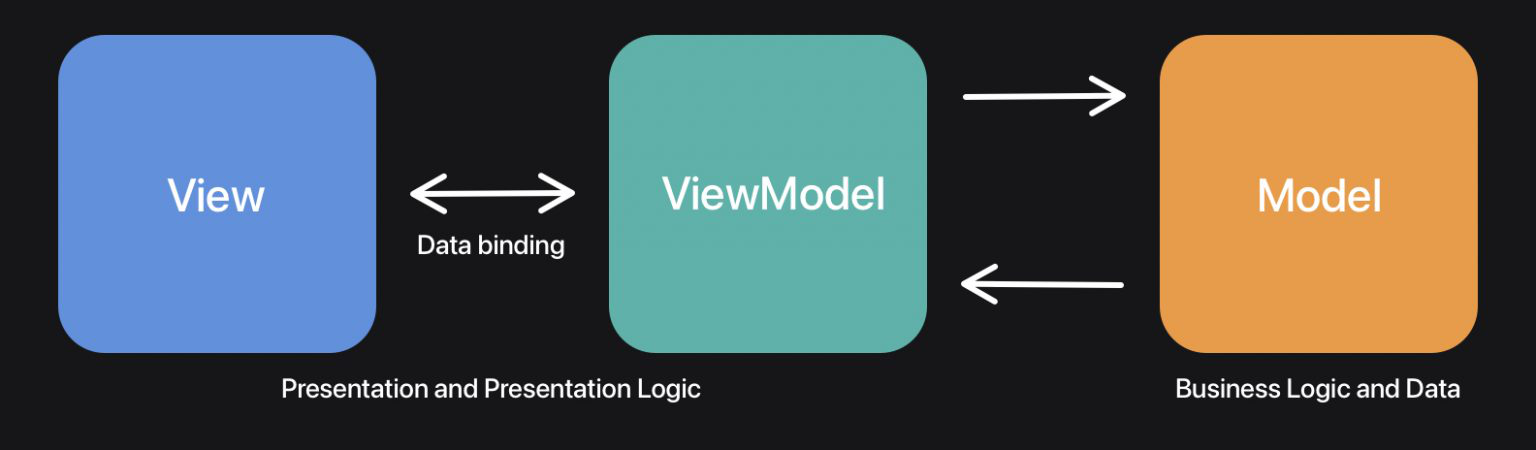
\includegraphics[width=150mm, keepaspectratio]{figures/MVVM-architectural-pattern.png}
    \caption{MVVM minta. \cite{MVVMArchitecture}}
    \label{fig:MVVMArchitecture}
\end{figure}

Ezek közül a legegyszerűbb a \textbf{Model réteg}. (\ref{lst:Model}.~kódrészlet)  
Ennek egyetlen célja az adatok tárolása a memóriában.  
Célszerű ezt olyan formában megtenni, ami már nem igényel sok átalakítást a köztes, ViewModel rétegben.  
Az adatok gyakran valamilyen REST API-ból érkeznek, tehát egy másik szoftvertől.  
Ehhez úgynevezett DTO-kat (data transfer object) használunk, az én programomban ezek lényegében megegyeznek a modellekkel, mivel kifejezetten erre készült a REST API.  
Természetesen így is van szükség egyéb data class-okra, vagyis valós modellekre. A UI-nak szüksége lehet egyéb értékekre, például arra, hogy megfelelő módon van-e kitöltve létrehozás során az objektum, vagy sem.  
Továbbá az összetett elemek esetén a hivatkozásokat az UUID-kon keresztül fel kell oldani megjelenítés előtt. Ezt a szerepet általában már a ViewModel végzi el.  
Amennyiben nem saját adatforrást használunk, vagy komplexebb adatokat kapunk, érdemes külön modell osztályokat létrehozni, és csak a szükséges adatokkal tovább dolgozni.  
Ezt még a HTTP-kommunikációért felelős komponensben érdemes megtenni.

\begin{lstlisting}[caption={Egy DTO struktúrája. Szerializáció: \refstruc{sec:KotlinX}}, label={lst:Model}, language=Kotlin]
    import kotlinx.serialization.Serializable // Szerializáció

    @Serializable // Szerializációért felelős kódrész
    data class TopicDto(    // Kotlin data class
        val uuid: String = "",
        val topic: String,
        val description: String,
        val parentTopic: String = ""
    )
\end{lstlisting}

A leggyakoribb mód erre a HTTP-alapú kommunikáció, ahol az adatok JSON formátumban érkeznek.  
Elképzelhető erre más alternatíva, például az adatok XML formátumban érkeznek.  
Más módon működő rendszerek is lehetnek, például WebSocketek, ahol az első csatlakozás során kialakul egy kétirányú csatorna, ahol mind a szerver, mind a kliens tud kommunikációt kezdeményezni.  
IoT környezetben az MQTT protokollt szokás alkalmazni. "Ez egy pub/sub protokoll, amely kis csomagmérettel és alacsony sávszélességgel rendelkezik, így ideális korlátozott hálózatokhoz és alacsony feldolgozási teljesítményű eszközökhöz. Az MQTT képes kezelni a szakaszos hálózati kapcsolódást, és támogatja a szolgáltatásminőség-szinteket (QoS) a megbízható üzenettovábbítás biztosítása érdekében." \cite{RESTAPIAlternatives}  
Egy további megoldás a gRPC, ami valós alternatíva lehet a REST API kommunikációra ebben a környezetben is. "A gRPC egy nyílt forráskódú keretrendszer, amelyet a Google fejlesztett RPC API-k építésére. Lehetővé teszi a fejlesztők számára, hogy szolgáltatás-interfészeket definiáljanak, valamint kliens- és szerveroldali kódot generáljanak, több programozási nyelven. A gRPC protokoll buffereket és nyelvfüggetlen adat-szerializációs formátumot használ a hatékony adatátvitel érdekében, ami ideálissá teszi magas teljesítményt igénylő alkalmazások számára. A gRPC nem feltétlenül a legjobb választás nagy mennyiségű adatmanipulációhoz vagy olyan alkalmazásokhoz, amelyek széleskörű kliens támogatást igényelnek. Ugyanakkor a gRPC magas teljesítményéről és alacsony erőforrásigényéről ismert, így jó választás azokhoz az alkalmazásokhoz, amelyek gyors és hatékony kommunikációt igényelnek a szolgáltatások között." \cite{RESTAPIAlternatives}

A köztes szinten a \textbf{ViewModel} található.  
Megoldáshoz az Android ViewModel Kotlin Multiplatform implementációját használtam fel (\refstruc{sec:ViewModel}), de bármi hasonló megoldás megfelel.  
Ennek a rétegnek számos feladata van.  
Az adatok lekérdezése itt valósul meg. Úgynevezett coroutine-scope-okban kezdeményezhetünk hosszabb ideig tartó függvényhívásokat.  
"A Kotlin standard könyvtára csak minimális alacsony szintű API-kat biztosít, hogy más könyvtárak használhassák a koroutine-kat. Ellentétben sok más hasonló képességű nyelvvel, az async és await nem kulcsszavak a Kotlinban, és még a standard könyvtár részei sem.  
Ezenkívül a Kotlin felfüggeszthető függvény (suspending function) koncepciója biztonságosabb és kevésbé hibára hajlamos absztrakciót kínál az aszinkron műveletekhez, mint a jövők (futures) és ígéretek (promises).  
A kotlinx.coroutines egy JetBrains által fejlesztett gazdag könyvtár koroutine-khoz. Számos magas szintű, koroutine-kompatibilis primitívet tartalmaz, amelyeket ez az útmutató is tárgyal, beleértve a launch, async és más függvényeket." \cite{Coroutine}  

Röviden összefoglalva: az aszinkron módon működő koroutine-k nem a UI-szálon hajtódnak végre, ezáltal nem blokkolják azt, és a felhasználói felület reszponzív marad a teljes idő alatt.  
Mindebből következik, hogy a REST API service hívásai innen indulnak, majd kerülnek bele State-ekbe vagy StateFlow-kba (\refstruc{sec:State}).  
Egy érdekesebb megközelítés a LiveData. Ez az eszköz az Observer mintát valósítja meg.  
Amennyiben például egy WebSocket alapú megoldást választottam volna, akkor a szerver automatikusan tudna üzenetet küldeni, amelyben leküldi az új adatot a kliensnek, és egyéb frissítés nélkül megjelenne az új adat.  
Ez egy példa a Model -> ViewModel -> View irányra. A legtöbb chat applikáció (például Messenger) is hasonló megközelítést alkalmazhat.

A ViewModelnek további feladatai közé tartozik az adatok transzformálása.  
Szükség lehet a hivatkozások feloldására; például egy kérdés esetén nem egy UUID-t szeretne a felhasználó látni a pont és a téma mezőkben, hanem azok neveit.  
Ezen kívül biztosíthat egyéb függvényeket az adatok módosítására, tovább navigálásra vagy bármilyen általános célokra.  
Ezzel elkerülhető, hogy logikát leíró kódot a View-n kelljen definiálni; elég egy összefogó részben levő függvényt meghívni. (\ref{lst:TransformationAndFunction}.~kódrészlet)

\begin{lstlisting}[caption={Példa a DTO átalakítására a valós UI-n használt modellé és egy példa logikát leíró függvényre. Az eredeti DTO: \ref{lst:Model}.~kódrészlet}, label={lst:TransformationAndFunction}, language=Kotlin]
data class TopicDetails(
    val id: String = "",
    val topic: String = "",
    val parent: String = "",            // Ez itt még egy UUID
    val description: String = "",
    val parentTopicName : String = ""   // Itt már fel lett oldva, ez fog a UI-on megjelenni
)

fun TopicDetails.toTopic(): TopicDto = // Ez egy extension function, ami visszaalakítja a UI-n megjelenő adatot a REST API által kezelhető formára
    TopicDto(
        uuid = id,
        topic = topic,
        parentTopic = if (parent == "null") "" else parent,
        description = description,
    )

// A névfeloldott változat kiegészül egy valid mezővel, mivel ez egy szerkeszthető nézethez tartozó modell lesz
fun TopicDto.toTopicUiState(isEntryValid: Boolean = false, parentName: String): TopicUiState = TopicUiState(
    topicDetails = this.toTopicDetails(parentName),
    isEntryValid = isEntryValid
)

// Biztosított függvény az adatok módosítására
fun updateUiState(topicDetails: TopicDetails) {
    topicUiState =
        TopicUiState(topicDetails = topicDetails, isEntryValid = validateInput(topicDetails))
}
\end{lstlisting}



A \textbf{View} a megjelenítési réteg, a felhasználó ezzel a résszel tud közvetlenül interakcióba lépni.  
Általános működési elve a következő: amikor a felhasználó az adott képernyőre navigál, a ViewModel betölti az adatokat.  
Ezt követően a felhasználó szabadon végezhet műveleteket rajta (\ref{lst:ExampleUI}.~kódrészlet). Ahogy a \ref{fig:UsecaseDiagram}.~ábrán is látható, megtekintheti az adott oldalt, esetenként törölheti vagy szerkesztheti az adatokat, illetve felvehet újat.  
Ezeket a funkciókat a megfelelő ViewModel-beli függvény meghívásával érhetjük el, és valamely felhasználói interakció váltja ki, például egy gomb megnyomása.  

\begin{lstlisting}[caption={Egy a View rétegbe tartozó felület leírásának részlete}, label={lst:ExampleUI}, language=Kotlin, float]
@Composable
private fun NewTopicScreenUiState(
    viewModel: TopicEntryViewModel, ...     // A használt ViewModel
) {
    ...
    Scaffold(...) { innerPadding ->
        TopicEntryBody(
            topicUiState = viewModel.topicUiState,          // A megjelenítendő UI adat
            onTopicValueChange = viewModel::updateUiState,  // ViewModelben definált függvény paraméterként való átadása
            onSaveClick = {
                coroutineScope.launch {                     // Aszinkron módon történő hívás, mentés funkció. Szintén a ViewModel függvényét hívja meg
                    if (viewModel.saveTopic()) {
                        navigateBack()
                    } else {
                        showNotify = true
                        notifyMessage = "Topic with this name already exists"
                    }
                }
            },
            modifier = Modifier                             // Fontos az igényes megjelenítés
                .padding(innerPadding)
                .verticalScroll(rememberScrollState())
                .fillMaxWidth()
        )
    }
}
\end{lstlisting}


Összefoglalva az MVVM tervezési mintát azt lehet mondani, hogy nagyon hatékonyan használható, és önmagában ezzel jelentősen növelhető a kód újrafelhasználhatósága.  
A mai lehetőségeket kihasználva a Compose Multiplatform területén ViewModeleket, DTO-kat és Modeleket elegendő egyszer, a commonMain alatt létrehozni és megvalósítani.
Az alkalalmazás betöltése is rögtön ezt a megoldást hasznnálja (\ref{lst:Start}.~kódrészlet)
Az ezekhez tartozó esetleges függvényeket, amennyiben szükség van rá, elegendő egy actual/expect párral lecserélni; nálam a kamera és a PDF exportálás is így működik. (\ref{lst:ExpectActualSample}.~kódrészlet)  
Az \textbf{expect/actual tervezési elv} működik minden rétegben, de általában csak a UI és néhány specifikus funkció megvalósítására van szükség a logika megvalósításához.  
Ilyenkor is elég egy közös ViewModel, és a build rendszer behelyettesíti a megfelelő függvényt a platformnak megfelelően.  


\begin{lstlisting}[caption={Egyszerűbb példa az expect és actual függvények használatára. Debugolás során használt kódrészlet.}, label={lst:ExpectActualSample}, language=Kotlin]
    //Közös függvény fejléc, lehet alapértelmezett paramétere is.
    @Composable
    internal expect fun Notify(message: String)
    
    
    //Android megvalósítás.
    @Composable
    internal actual fun Notify(message: String) {
        Toast.makeText(
            LocalContext.current, message, Toast.LENGTH_SHORT
        ).show()
    }
    
    //Asztali alkalmazás megvalósítása.
    @Composable
    internal actual fun Notify(message: String) {
        if (SystemTray.isSupported()) {
            val tray = SystemTray.getSystemTray()
            val image = Toolkit.getDefaultToolkit().createImage("logo.webp")
            val trayIcon = TrayIcon(image, "Desktop Notification")
            tray.add(trayIcon)
            trayIcon.displayMessage("Desktop Notification", message, TrayIcon.MessageType.INFO)
        } else {
            ...
        }
    }
\end{lstlisting}

\pagebreak

\begin{lstlisting}[caption={Alkalamzás elindítása}, label={lst:Start}, language=Kotlin]
    // Tipikus Android compose alkalamzás. (androidMain)
    class MainActivity : ComponentActivity() {
        override fun onCreate(savedInstanceState: Bundle?) {
            super.onCreate(savedInstanceState)
            setContent {
                App()
            }
        }
    }
    
    //Kotlin swing alkalmazás. (desktopMain)
    fun main() = application {
        Window(
            onCloseRequest = ::exitApplication,
            title = "Exam App",
        ) {
            App()
        }
    }
    
    //A hívott közös kód. (commonMain)
    @Composable
    fun App() {
        MaterialTheme {
            NavigationComponent()
        }
    }
\end{lstlisting}


A másik legfontosabb architekturális elem a UIState használata. (\ref{lst:UiState}.~kódrészlet)  
Ezzel a mintával egyszerűen kezelhető több fajta képernyő ugyanazon az oldalon.  
A megvalósítása sealed interfészek segítségével történik, így a Kotlinban a switch-case szerkezetnek megfeleltethető `when` használatával egyszerűen válthatunk közöttük.  
Ebben a mintában gyakran három állapota van a képernyőnek: loading, success és error.  

A hosszú ideig tartó HTTP-kérések ideje alatt így egy töltőképernyőt mutathatunk egy látszólag lefagyott vagy hiányos oldal helyett.  
Az adatok megérkezése után átadhatjuk azokat a Success képernyőnek, hiba esetén pedig megjeleníthetjük a hiba képernyőt, ahol található valamilyen magyarázat a felhasználó számára, például "Nem sikerült betölteni a kért oldalt, mert a hálózat állapota nem megfelelő".  

\begin{lstlisting}[caption={UiState megvalóstása}, label={lst:UiState}, language=Kotlin]
sealed interface TopicDetailsScreenUiState {
    data class Success(val point: TopicDto) : TopicDetailsScreenUiState
    data object Error : TopicDetailsScreenUiState{var errorMessage: String = ""}
    data object Loading : TopicDetailsScreenUiState
}
\end{lstlisting}



A képernyő állapotát a ViewModelből lehet szabályozni, ahol felveszünk erre egy State-et. A képernyőre navigálás során az alapértelmezett érték a töltés.  
Az adatok megérkezése után a State-ben beállítjuk a megfelelő értéket, és a View erről kap egy értesítést, amelynek hatására lefut a recomposition. Ennek eredményeként megjelenik az új nézet.  
(\ref{lst:UiStateSetting}.~kódrészlet) 

\begin{lstlisting}[caption={UiState beállítása}, label={lst:UiStateSetting}, language=Kotlin, float]
var topicDetailsScreenUiState: TopicDetailsScreenUiState by mutableStateOf(TopicDetailsScreenUiState.Loading) // State alap loading értékkel
fun getTopic(topicId: String){
    topicDetailsScreenUiState = TopicDetailsScreenUiState.Loading   // Ha nem lenne beállítva beállítjuk a loadingot
    viewModelScope.launch { // Aszinkron hívás környezete, így a loading animációt nemblokkoljuk
        topicDetailsScreenUiState = try{    // Az eredméyn megérkezése után vagy mutatjuk az adatot...
            val result = ApiService.getTopic(topicId)
            ...
        TopicDetailsScreenUiState.Success(result)
        } catch (e: ApiException) { // ...vagy egy hiba képernyőt
            TopicDetailsScreenUiState.Error.errorMessage = e.message ?: "Unkown error"
            TopicDetailsScreenUiState.Error
        } 
    }
}
\end{lstlisting}

Összefoglalva ezt a mintát: a felhasználót aktívan tudjuk tájékoztatni a program állapotáról.  
A töltőképernyő miatt tudni fogja, hogy a háttérben tart az adatok betöltése, és nem lesz olyan érzése, mintha lefagyott volna az alkalmazás.  
Hiba esetén is tudunk tájékoztatást adni, így lehetőséget biztosítunk a felhasználónak arra, hogyha nála van a hiba (például nincs internet), akkor megoldja, vagy esetlegesen jelezze a problémát a megadott elérhetőségen. A megjelenített információ miatt ezt viszonylag pontosan meg tudja tenni.  
Ezek hatására a felhasználói élmény jelentősen javulhat.

\section{Rendszer felépítései, komponensei}
\label{sec:Components}

Ebben az alfejezetben komponensdiagramokon keresztül mutatom be az alkalmazást.  
Először adok egy általános nézetet, majd a fontosabb, több tartalommal rendelkező egységeket a kisebb alegységeit is bemutatom.  

"Az UML komponensdiagramokat az objektumorientált rendszerek fizikai aspektusainak modellezésére használják, amelyek célja a komponensalapú rendszerek vizualizálása, specifikálása és dokumentálása, valamint végrehajtható rendszerek létrehozása előre- és visszafelé történő tervezéssel. A komponensdiagramok lényegében osztálydiagramok, amelyek a rendszer komponenseire összpontosítanak, és gyakran a rendszer statikus implementációs nézetének modellezésére használják." \cite{ComponentDiagram}  

Ebből az idézetből kiderül, hogy ebben a diagramtípusban a fizikai egységek jelennek meg.  
Ezt érthetjük szó szerint is, például más gépen futó backend és frontend, de akár önálló fordítási egységet is érthetünk alatta.  
Ilyen önálló egység lehet a business logic réteg; .NET környezetben ez egy teljesen általános megoldás, ahol valódi fordítási egységet alkot, és önálló DLL jön belőle létre.  
Hasonló módon foghatjuk fel a Compose Multiplatformban szereplő közös és specifikus kódokat is.  

\subsection{Általános komponensek felépítése}

Két fő komponensből áll az alkalmazás, a Compose Multiplatform applikációból és az adatokat kiszolgáló REST API-ból. (\refstruc{fig:ComponentDiagram})  
Ebben a félévben a kliens oldalon volt a hangsúly, ezért a backend részt nem bontom fel további részekre, kezelhetjük egyfajta \emph{"black box"}-ként.  

A kliens oldalon a business logic komponens kommunikál a backenddel, így függ tőle. Az abban történő változás vagy hiba kihat ennek a komponensnek a működésére.  
Többek között ebben az egységben találhatóak a ViewModelek és a Servicek közé sorolt funkciók.  

A Common Client rész tartalmazza a View réteget.  
Itt találhatóak a Composable függvényekkel leírt képernyők.  
Mivel ezeken az elemeken a ViewModelből származó adatok jelennek meg a helyes működés szerint, ezért függ a business logictól.  
Ezáltal tranzitívan függ a backend helyes működésétől is.  
Ennek a felépítéséről és komponenseiről lesz egy részletesebb ábra.  

Megjelennek még az ábrán a Mobile Client és Desktop Client részek is.  
Ez a két komponens valósítja meg a platformspecifikus kódrészleteket, és felel a belépési pontok megvalósításáért.  
Itt is érdemes észrevenni, hogy ezek a komponensek függnek a közös kódtól.  
Ha megváltozik valami benne, az minden platformspecifikus kódra hatással lesz; ha létrehozunk egy expect függvényt, azt minden más komponensben meg kell valósítani.  
Ezekről ebben a fejezetben nem fogok részletesebben foglalkozni.  


\begin{figure}[!ht]
    \centering
    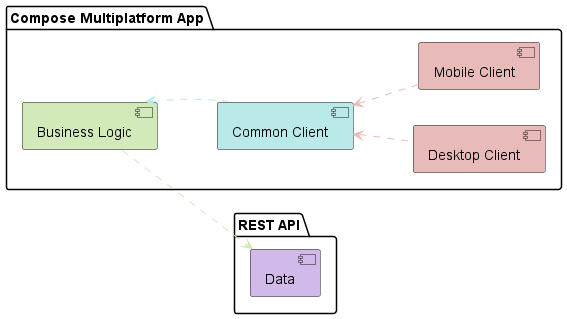
\includegraphics[width=150mm, keepaspectratio]{figures/Component.png}
    \caption{Átfogó komponens diagram.}
    \label{fig:ComponentDiagram}
\end{figure}

\subsection{Business logic komponensek felépítése}

A \textbf{bussines logic komponens} összetett és több alkotóelemből épül fel. (\refstruc{fig:BusinessComponentDiagram})
A ViewModelek önmagukban lehetnek komponensek, akár külön-külön is, de a diagramon egybe tüntetem fel.
Ezek a viewModelek függnek a Servicektől. 

A Serviceek közé tartozik az API kommunikáció, a navigáciért felelős komponens is.
A PDF elkészítéséért felelős kódrészek is egy komponensként kezelhető, hasonló módon, mint a szövegfelismerésért felelős funkció is.
Az ebben az egységebn levő komponensek nagyrészt nem függnek szorosan más komponensektől, ez alól kivétel a HTTP kommunikáció ami a backendtől függ.


\begin{figure}[!ht]
    \centering
    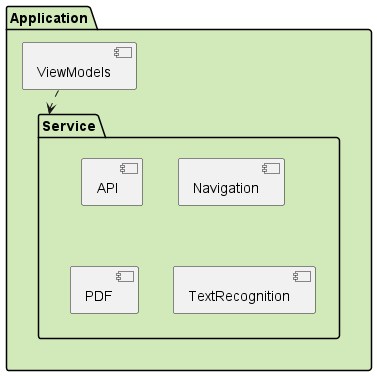
\includegraphics[width=100mm, keepaspectratio]{figures/Business Component.png}
    \caption{Business logic komponens diagram.}
    \label{fig:BusinessComponentDiagram}
\end{figure}

\subsection{Common Client komponensek felépítése}

A \textbf{common Client komponens} is számos részből épül fel. (\refstruc{fig:CommonComponentDiagram})
Ebben a részben találhatóak a képernyőn megjelenő elemek leírásásért felelős részek.

A kisebb komponenseket tartalmazó résztőll több másik is függ, ez az ábrán az átláthatósag miatt nem szerepel.
Egy-egy ilyen UI komponens egy vagy több viewModeltől is függhet, de egymás között nincs egyéb függőség, így szabadan eltávilíthatóak vagy hozzáadhatóak új nézetek.

Ezektől a komponensektől a tényleges implementációk függnek, így a Mobil és asztali komponens is.
Az itt történt bármilyen változás kihatással van a valós implementációkra.
A közös elemek módosítása megváltoztatja minden platformon a képernyő kinézetét.
Ha új expect függvényt veszünk fel, a többi kompenenst is külön el kell készítenünk.


\begin{figure}[!ht]
    \centering
    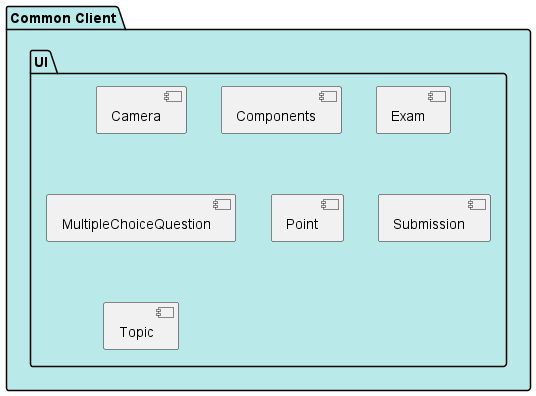
\includegraphics[width=100mm, keepaspectratio]{figures/Common Component.png}
    \caption{Közös UI komponens diagram.}
    \label{fig:CommonComponentDiagram}
\end{figure}